\documentclass[11pt,a4paper]{article}

\usepackage[utf8]{inputenc}
\usepackage[T1]{fontenc}
\usepackage{lmodern}
\usepackage[margin=2.5cm]{geometry}
\usepackage{amsmath,amssymb}
\usepackage{graphicx}
\usepackage{float}
\usepackage{booktabs}
\usepackage{caption}
\usepackage{subcaption}
\usepackage{xcolor}
\usepackage{listings}
\usepackage{hyperref}

\graphicspath{{figures/}}

\hypersetup{colorlinks=true, linkcolor=blue!60!black, urlcolor=blue!60!black}

% Non-ASCII characters in the code (e.g. hats in plot titles) are written with (* ... *)
\lstset{
  language=Python,
  basicstyle=\ttfamily\footnotesize,
  keywordstyle=\color{blue!70!black}\bfseries,
  commentstyle=\color{green!45!black}\itshape,
  stringstyle=\color{red!60!black},
  numbers=left,
  numberstyle=\tiny\color{gray},
  numbersep=6pt,
  frame=single,
  rulecolor=\color{gray!60},
  breaklines=true,
  breakatwhitespace=false,
  postbreak=\mbox{\textcolor{gray}{$\hookrightarrow$}\space},
  showstringspaces=false,
  columns=fullflexible,
  keepspaces=true,
  upquote=true,
  escapeinside={(*}{*)},
  captionpos=t
}

\newcommand{\todo}[1]{\textcolor{red}{\textbf{[TODO: #1]}}}

\title{OVM Homework Exercises I (WI3405TU)}
\author{\todo{Name} \\ \todo{Student number}}
\date{October 2026}

\begin{document}
\maketitle

\noindent All computations were done in Python (\texttt{numpy}, \texttt{scipy}, \texttt{pandas},
\texttt{matplotlib}, \texttt{yfinance}). The full annotated code is given in
Appendix~\ref{app:code} and is also submitted separately as \texttt{OVM\_assignment\_1.ipynb}.

%======================================================================
\section{Market stock prices}
%======================================================================

The Apple (AAPL) close prices were downloaded with the \texttt{yfinance} package
(Listing~\ref{lst:q1a-price}).

\subsection*{(a) Prices and returns}

\paragraph{Price movement.} Figure~\ref{fig:q1a-close} shows the daily close price from
1 September 2025 to 31 August 2026.

\begin{figure}[H]
  \centering
  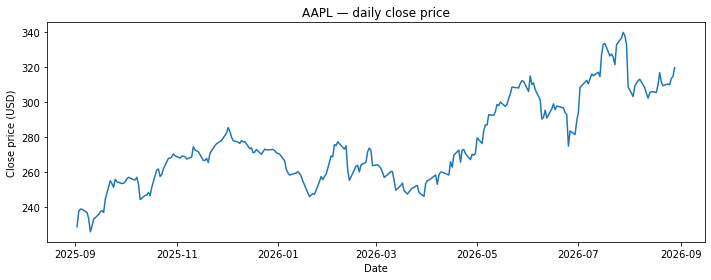
\includegraphics[width=0.9\textwidth]{q1a_close.png}
  \caption{AAPL daily close price, 1 September 2025 -- 31 August 2026.}
  \label{fig:q1a-close}
\end{figure}

\paragraph{Daily returns.} With $S_i$ the close price on day $i$ we compute the simple and
logarithmic returns
\[
  r_i = \frac{S_i - S_{i-1}}{S_{i-1}}, \qquad
  \hat r_i = \ln\!\left(\frac{S_i}{S_{i-1}}\right)
\]
(Listing~\ref{lst:q1a-returns}). Both series are shown in Figure~\ref{fig:q1a-returns}.

\begin{figure}[H]
  \centering
  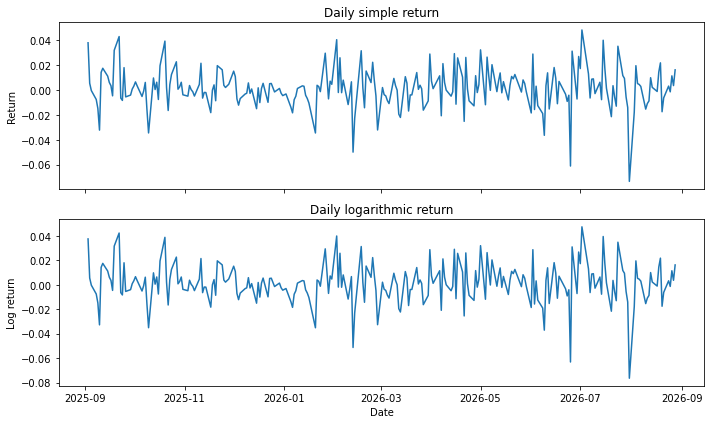
\includegraphics[width=0.9\textwidth]{q1a_returns.png}
  \caption{Daily simple returns (top) and daily logarithmic returns (bottom).}
  \label{fig:q1a-returns}
\end{figure}

\paragraph{When are the two returns approximately identical?} The two returns are related by
$\hat r_i = \ln(1 + r_i)$. A Taylor expansion around $r_i = 0$ gives
\[
  \hat r_i = r_i - \frac{r_i^2}{2} + \frac{r_i^3}{3} - \dots ,
\]
so $\hat r_i \approx r_i$ whenever the relative price change $|r_i|$ is small, i.e.\ when the
price changes little between two consecutive observations (short time steps, low volatility).
The difference is of order $r_i^2/2$. For typical daily moves of about $1$--$2\%$ this is only
$10^{-4}$, which is why the two panels in Figure~\ref{fig:q1a-returns} are practically
indistinguishable. Since $\ln(1+x) \le x$, the log return is always slightly smaller than the
simple return, and the gap only becomes visible on days with large moves (e.g.\ the
$\approx -7\%$ day at the end of July 2026). For longer horizons (monthly, yearly) or very
volatile assets the approximation breaks down.

\subsection*{(b) Statistics}

\paragraph{Daily data (1 year).} The histogram of the daily log returns is shown in
Figure~\ref{fig:q1b-hist-daily} (Listing~\ref{lst:q1b-hist}). The sample mean and variance are
\[
  \hat\mu = 0.0013422, \qquad \hat\sigma^2 = 0.00025250 \quad (\hat\sigma = 0.01589).
\]
Figure~\ref{fig:q1b-qq-daily} compares the empirical quantiles with the quantiles of
$\mathcal N(\hat\mu, \hat\sigma^2)$ (Listing~\ref{lst:q1b-qq}). The quantiles were computed
directly: the sorted returns are plotted against $\Phi^{-1}_{\hat\mu,\hat\sigma}\big((k-0.5)/n\big)$,
$k = 1,\dots,n$.

\begin{figure}[H]
  \centering
  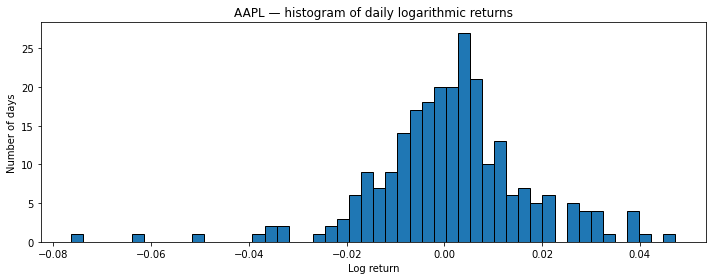
\includegraphics[width=0.85\textwidth]{q1b_hist_daily.png}
  \caption{Histogram of daily logarithmic returns, 1 September 2025 -- 31 August 2026.}
  \label{fig:q1b-hist-daily}
\end{figure}

\begin{figure}[H]
  \centering
  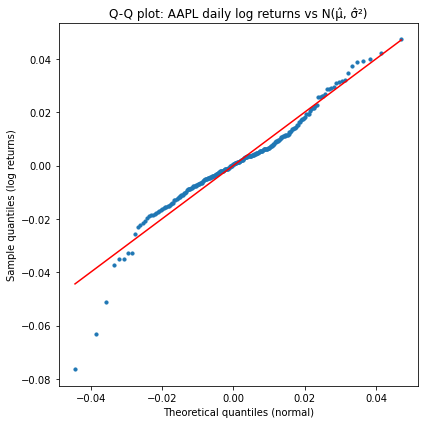
\includegraphics[width=0.5\textwidth]{q1b_qq_daily.png}
  \caption{Q-Q plot of daily log returns (1 year) against $\mathcal N(\hat\mu, \hat\sigma^2)$.}
  \label{fig:q1b-qq-daily}
\end{figure}

\paragraph{Weekly data (2022--2025).} The same procedure was repeated for the weekly close
prices over the four years 2022--2025 (Listing~\ref{lst:q1b-weekly}). For a fair comparison over
the same period, the daily Q-Q plot was also redone for 2022--2025. The weekly log returns have
\[
  \hat\mu_w = 0.0022960, \qquad \hat\sigma_w^2 = 0.0014772 \quad (\hat\sigma_w = 0.03843),
\]
and the daily log returns over 2022--2025 have $\hat\mu_d = 0.0004260$,
$\hat\sigma_d^2 = 0.0003205$ ($\hat\sigma_d = 0.01790$).

\begin{figure}[H]
  \centering
  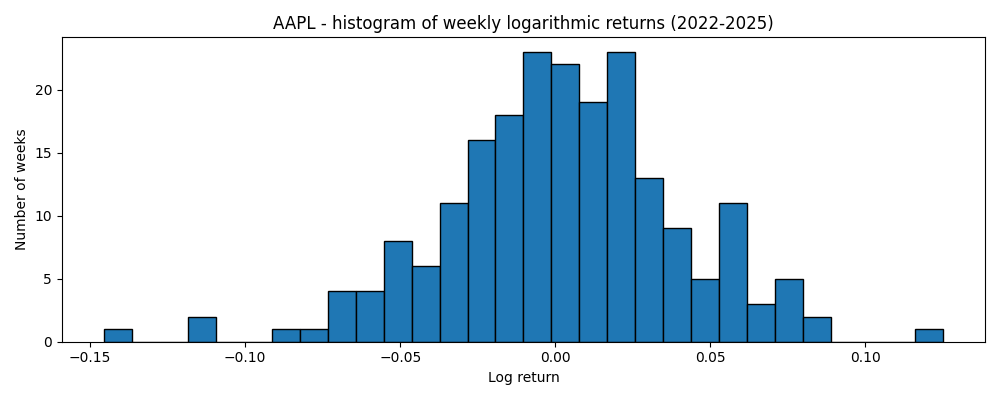
\includegraphics[width=0.85\textwidth]{q1b_hist_weekly.png}
  \caption{Histogram of weekly logarithmic returns, 2022--2025.}
  \label{fig:q1b-hist-weekly}
\end{figure}

\begin{figure}[H]
  \centering
  \begin{subfigure}{0.48\textwidth}
    \centering
    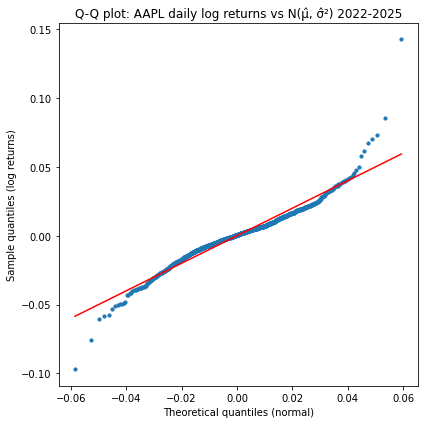
\includegraphics[width=\textwidth]{q1b_qq_daily_2022_2025.png}
    \caption{Daily log returns, 2022--2025.}
  \end{subfigure}
  \hfill
  \begin{subfigure}{0.48\textwidth}
    \centering
    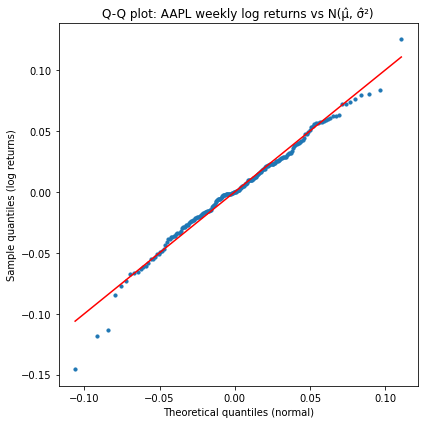
\includegraphics[width=\textwidth]{q1b_qq_weekly.png}
    \caption{Weekly log returns, 2022--2025.}
  \end{subfigure}
  \caption{Q-Q plots against the fitted normal distributions.}
  \label{fig:q1b-qq-compare}
\end{figure}

\paragraph{Comparison.} The daily Q-Q plots (Figures~\ref{fig:q1b-qq-daily} and
\ref{fig:q1b-qq-compare}a) have the typical S-shape of a heavy-tailed distribution: the points
lie close to the line in the centre, but bend below it in the left tail and above it in the right
tail. Extreme daily moves (up to $-10\%$ and $+14\%$ in 2022--2025) are much more frequent than a
normal distribution predicts, and the centre of the distribution is more peaked. The weekly Q-Q
plot (Figure~\ref{fig:q1b-qq-compare}b) follows the line much more closely and only deviates for
a handful of extreme weeks. This is consistent with the central limit theorem: a weekly log
return is the sum of about five daily log returns, so its distribution is closer to normal. The
normal (log-normal price) model is therefore a better description at the weekly scale than at
the daily scale. Note also that $\hat\mu_w \approx 5.4\,\hat\mu_d$ and
$\hat\sigma_w^2 \approx 4.6\,\hat\sigma_d^2$, roughly as expected when weekly returns are sums of
about five independent daily returns.

%======================================================================
\section{Monte Carlo}
%======================================================================

\paragraph{Exact value and variance.} For $U \sim \mathcal U(0,1)$,
\[
  \mathbb E\!\left[\frac{1}{\sqrt U}\right] = \int_0^1 u^{-1/2}\,du = \big[2\sqrt u\,\big]_0^1 = 2,
  \qquad
  \mathbb E\!\left[\Big(\frac{1}{\sqrt U}\Big)^2\right] = \int_0^1 \frac{du}{u} = \infty .
\]
So $Y = 1/\sqrt U$ has a finite mean but an \emph{infinite variance}. This is the key point of
the exercise: the standard CLT, which gives errors of order $\sigma/\sqrt N$ and asymptotically
normal errors, does not apply directly.

\paragraph{Basic estimate.} With $N = 1000$ samples (Listing~\ref{lst:q2-basic}) the Monte Carlo
estimate $\frac1N\sum_{k=1}^N U_k^{-1/2}$ is $2.0108$, an absolute error of $0.0108$.

\paragraph{Estimates and confidence intervals.} For $N = 10^2, 10^3, 10^4, 10^5$ we computed one
estimate and its usual 95\% confidence interval $\hat\mu \pm 1.96\,s/\sqrt N$
(Listing~\ref{lst:q2-ci}). The results are in Table~\ref{tab:q2-ci} and
Figure~\ref{fig:q2-ci}.

\begin{table}[H]
  \centering
  \begin{tabular}{rcc}
    \toprule
    $N$ & Estimate & 95\% CI \\
    \midrule
    $10^2$ & 1.6596 & $[1.5144,\ 1.8048]$ \\
    $10^3$ & 2.0020 & $[1.8592,\ 2.1448]$ \\
    $10^4$ & 2.0156 & $[1.9600,\ 2.0712]$ \\
    $10^5$ & 1.9900 & $[1.9730,\ 2.0069]$ \\
    \bottomrule
  \end{tabular}
  \caption{Monte Carlo estimates of $\mathbb E[1/\sqrt U] = 2$ with 95\% confidence intervals.}
  \label{tab:q2-ci}
\end{table}

\begin{figure}[H]
  \centering
  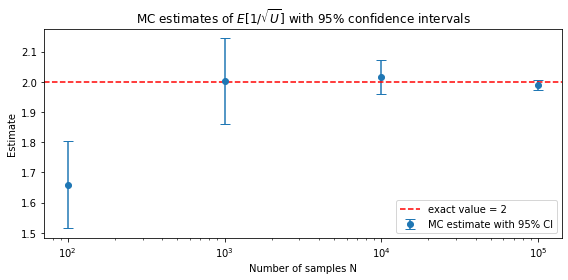
\includegraphics[width=0.8\textwidth]{q2_ci.png}
  \caption{MC estimates with 95\% confidence intervals for different sample sizes.}
  \label{fig:q2-ci}
\end{figure}

\paragraph{Speed of convergence and CI coverage.} To study the distribution of the error, the
experiment was repeated $M = 1000$ times for every $N$ (Listing~\ref{lst:q2-repeat}).
Table~\ref{tab:q2-conv} lists the mean absolute error and the fraction of the $M$ confidence
intervals that contain the true value 2. The mean absolute error is plotted against $N$ in
Figure~\ref{fig:q2-conv}.

\begin{table}[H]
  \centering
  \begin{tabular}{rcc}
    \toprule
    $N$ & Mean $|$error$|$ & Coverage of 95\% CI \\
    \midrule
    $10^2$ & 0.17670 & 0.851 \\
    $10^3$ & 0.06886 & 0.898 \\
    $10^4$ & 0.02989 & 0.924 \\
    $10^5$ & 0.00954 & 0.935 \\
    \bottomrule
  \end{tabular}
  \caption{Mean absolute error and empirical CI coverage over $M = 1000$ repetitions.}
  \label{tab:q2-conv}
\end{table}

\begin{figure}[H]
  \centering
  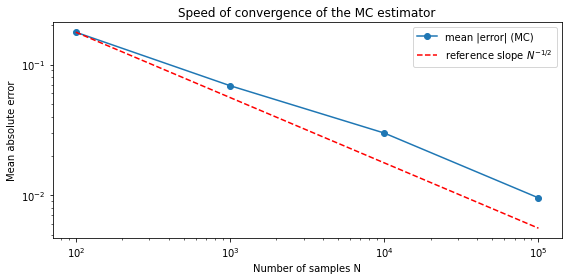
\includegraphics[width=0.8\textwidth]{q2_convergence.png}
  \caption{Mean absolute error versus $N$ (log-log scale) with a reference slope $N^{-1/2}$.}
  \label{fig:q2-conv}
\end{figure}

\paragraph{Normality of the errors.} Figure~\ref{fig:q2-normality} shows, for each $N$, the
histogram of the $M = 1000$ errors with the fitted normal density, and the Q-Q plot of the errors
against that normal distribution (Listing~\ref{lst:q2-normality}).

\begin{figure}[H]
  \centering
  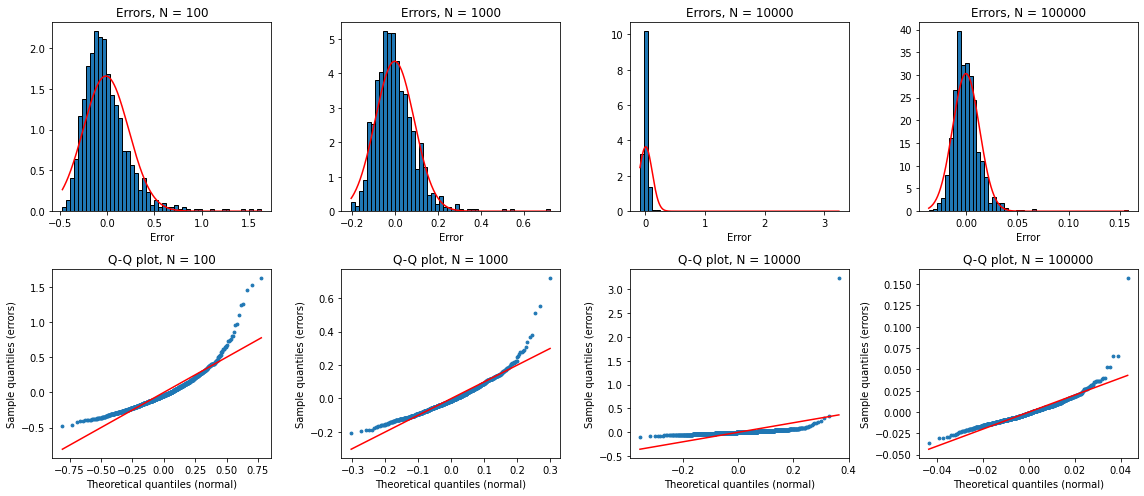
\includegraphics[width=\textwidth]{q2_normality.png}
  \caption{Top: histograms of the MC errors with the fitted normal density. Bottom: Q-Q plots of
  the errors against the fitted normal distribution.}
  \label{fig:q2-normality}
\end{figure}

\paragraph{Discussion.}
\begin{itemize}
  \item \textbf{Speed of convergence.} The estimates get closer to 2 as $N$ grows and the
  confidence intervals become narrower. On the log-log plot the mean absolute error follows the
  reference slope $N^{-1/2}$ closely, but over each tenfold increase of $N$ it decreases by a
  factor of $2.3$--$3.1$, slightly less than $\sqrt{10} \approx 3.16$. This is caused by the
  infinite variance. Since $P(Y > y) = P(U < y^{-2}) = y^{-2}$, $Y$ lies exactly on the border
  of the domain of attraction of the normal law. The generalised CLT then gives an error of order
  $\sqrt{\ln N / N}$ instead of $1/\sqrt N$, i.e.\ convergence that is only slightly slower than
  usual.

  \item \textbf{Normality of the errors.} Because the variance is infinite, the classical CLT
  does not apply directly. The histograms are clearly right-skewed with a long right tail: rare
  samples with very small $U$ produce huge values of $1/\sqrt U$ and pull the estimate up. The
  fitted normal density does not match the shape of the histogram. In the Q-Q plots the points
  bend away from the line in the right tail. This departure is strongest for $N = 10^2$ and
  becomes milder as $N$ grows. The errors do become asymptotically normal, but only very slowly
  (with the logarithmic correction above).

  \item \textbf{Confidence intervals.} Because the errors are not normal and the sample standard
  deviation $s$ underestimates the true spread (the true variance is infinite), the intervals
  $\hat\mu \pm 1.96\,s/\sqrt N$ contain the true value less often than 95\% of the time: from
  85\% for $N = 10^2$ up to 93.5\% for $N = 10^5$ (Table~\ref{tab:q2-conv}). These intervals
  should therefore be read with caution for this integrand. The infinite variance also makes $s$
  unstable: one very small $U$ can inflate it, so a larger $N$ does not always give a narrower
  interval in a single run.
\end{itemize}

%======================================================================
\section{Simulation of stock price paths}
%======================================================================

The parameters are $T = 1$, $S_0 = 170$, $\sigma = 0.344$, $\mu = 0.1$.

\subsection*{(a) Discrete price model}

The discrete model $S(t_{i+1}) = S(t_i)\big(1 + \mu\,\Delta t + \sigma\sqrt{\Delta t}\,Z_i\big)$,
$Z_i \sim \mathcal N(0,1)$, was simulated with $\Delta t = T/L$. Figure~\ref{fig:q3a-path} shows
one path for $L = 5$ (Listing~\ref{lst:q3a-path}). Repeating the simulation $M = 5000$ times and
storing $S_T$ gives the histogram in Figure~\ref{fig:q3a-hist} (Listing~\ref{lst:q3a-hist}).

\begin{figure}[H]
  \centering
  \begin{subfigure}{0.48\textwidth}
    \centering
    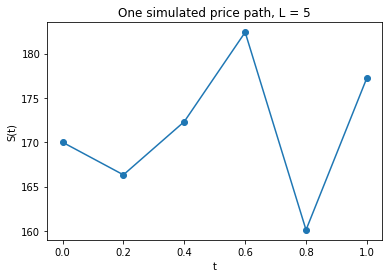
\includegraphics[width=\textwidth]{q3a_path.png}
    \caption{One simulated path, $L = 5$.}
    \label{fig:q3a-path}
  \end{subfigure}
  \hfill
  \begin{subfigure}{0.48\textwidth}
    \centering
    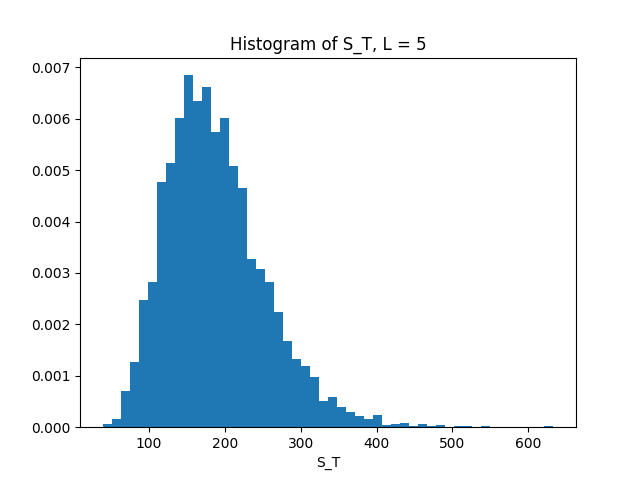
\includegraphics[width=\textwidth]{q3a_hist.png}
    \caption{Histogram of $S_T$, $L = 5$, $M = 5000$.}
    \label{fig:q3a-hist}
  \end{subfigure}
  \caption{Discrete price model with $L = 5$.}
\end{figure}

The simulation was repeated for $L = 5, 10, 20, 50, 100$ (Listing~\ref{lst:q3a-ecdf}). In
Figure~\ref{fig:q3a-ecdf} the empirical distribution functions of $S_T$ are compared with the
theoretical distribution function of the continuous-time model
$S_T = S_0 e^{(\mu - \frac12\sigma^2)T + \sigma\sqrt T Z}$, which is log-normal:
\[
  F(x) = P(S_T \le x) = \Phi\!\left(\frac{\ln(x/S_0) - (\mu - \frac12\sigma^2)T}{\sigma\sqrt T}\right).
\]

\begin{figure}[H]
  \centering
  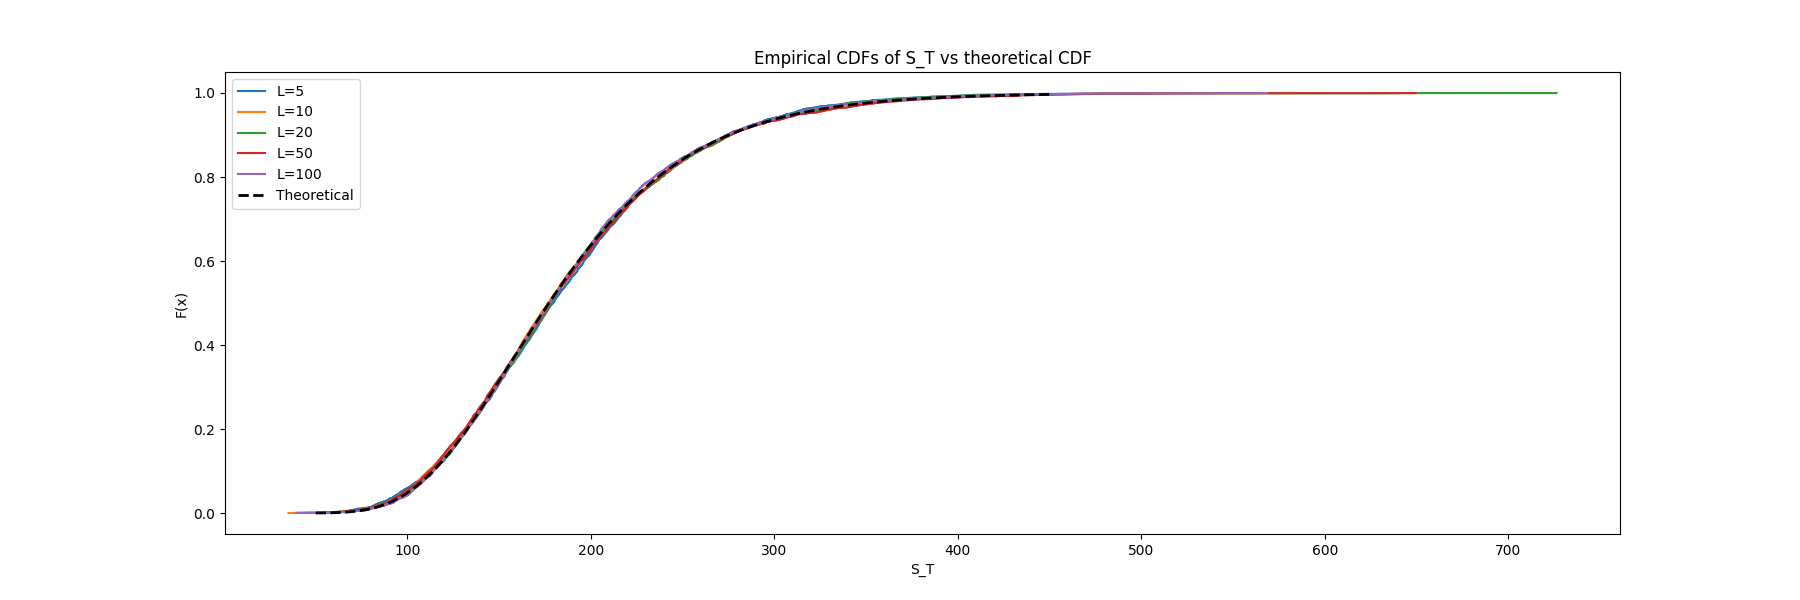
\includegraphics[width=\textwidth]{q3a_ecdf.png}
  \caption{Empirical distribution functions of $S_T$ for different $L$ ($M = 5000$) and the
  theoretical log-normal distribution function.}
  \label{fig:q3a-ecdf}
\end{figure}

All empirical distribution functions lie very close to the theoretical one. As $L$ increases, the
discrete model converges to the continuous geometric Brownian motion, and the empirical CDFs
approach the log-normal CDF. Already for $L = 5$ the difference is small, because the drift and
volatility over one year are moderate. With $L = 5$ the product of only five factors
$(1 + \mu\Delta t + \sigma\sqrt{\Delta t}Z_i)$ is less right-skewed than the log-normal, and a
factor can even become negative for large negative $Z_i$. These effects disappear as $L$ grows.
The remaining small wiggles of the curves are Monte Carlo noise from the finite $M$.

\subsection*{(b) Standard Monte Carlo vs.\ antithetic variables}

Using the exact continuous-time model, $\mathbb E[S_T]$ was estimated with standard Monte Carlo
from $M$ samples, and with antithetic variables from $M/2$ pairs $(Z, -Z)$, i.e.\ with the same
total number $M$ of evaluations of $S_T$:
\[
  \hat\mu_{AM} = \frac{2}{M}\sum_{k=1}^{M/2} \frac{S_T(Z_k) + S_T(-Z_k)}{2}.
\]
The exact value is $\mathbb E[S_T] = S_0 e^{\mu T} = 187.8791$. The results are in
Table~\ref{tab:q3b} (Listing~\ref{lst:q3b}).

\begin{table}[H]
  \centering
  \small
  \begin{tabular}{rccccc}
    \toprule
    $M$ & MC & 95\% CI (MC) & AMC & 95\% CI (AMC) & $I_M / I_{AM}$ \\
    \midrule
    $10^2$ & 181.234 & $[169.748,\ 192.719]$ & 186.090 & $[183.155,\ 189.025]$ & 3.913 \\
    $10^3$ & 188.182 & $[183.980,\ 192.384]$ & 188.386 & $[186.961,\ 189.811]$ & 2.949 \\
    $10^4$ & 187.746 & $[186.439,\ 189.052]$ & 187.520 & $[187.103,\ 187.938]$ & 3.127 \\
    $10^5$ & 187.667 & $[187.252,\ 188.081]$ & 187.889 & $[187.751,\ 188.027]$ & 3.005 \\
    \bottomrule
  \end{tabular}
  \caption{Estimates of $\mathbb E[S_T]$ with standard MC and antithetic MC (AMC), their 95\%
  confidence intervals and the ratio of the interval widths.}
  \label{tab:q3b}
\end{table}

Both methods converge to $187.879$ and every confidence interval contains the true value. For
the same $M$ the antithetic interval is about 3 times narrower. This agrees with theory. With
$m = \mathbb E[S_T]$,
\[
  \operatorname{Var}(S_T) = m^2\big(e^{\sigma^2 T} - 1\big), \qquad
  \operatorname{Cov}\big(S_T(Z), S_T(-Z)\big) = m^2\big(e^{-\sigma^2 T} - 1\big) < 0,
\]
so the ratio of the interval widths at equal cost is
\[
  \frac{I_M}{I_{AM}} = \sqrt{\frac{\operatorname{Var}(S_T)}{\operatorname{Var}(S_T) + \operatorname{Cov}(S_T(Z),S_T(-Z))}}
  = \sqrt{\frac{e^{\sigma^2 T} - 1}{e^{\sigma^2 T} + e^{-\sigma^2 T} - 2}} \approx 2.99 .
\]
The simulated ratios ($3.91$, $2.95$, $3.13$, $3.01$) scatter around this value. The scatter is
largest for $M = 10^2$, where the sample standard deviations themselves are noisy. The method
works well here because $S_T$ is a monotone, nearly linear function of $Z$ for moderate $\sigma$,
which makes $S_T(Z)$ and $S_T(-Z)$ strongly negatively correlated. Reducing the interval width by
a factor of 3 is equivalent to using about 9 times more samples with standard Monte Carlo.

%======================================================================
\section{Historical volatility}
%======================================================================

\subsection*{(a) Historical volatility}

The historical volatility is estimated from the sample standard deviation $s$ of the log returns
and annualised with $\hat\sigma = s/\sqrt{\Delta t}$, where $\Delta t = 1/252$ for daily and
$\Delta t = 1/52$ for weekly data (Listing~\ref{lst:q4a}). Both use the 2022--2025 data from
Question 1b.

\begin{table}[H]
  \centering
  \begin{tabular}{lcc}
    \toprule
    Data & $s$ (per period) & $\hat\sigma$ (annualised) \\
    \midrule
    Daily  & 0.01790 & 0.2842 \\
    Weekly & 0.03843 & 0.2772 \\
    \bottomrule
  \end{tabular}
  \caption{Historical volatility estimates of AAPL, 2022--2025.}
  \label{tab:q4a}
\end{table}

The two annualised estimates are very close (about 28\%), as expected if the log returns over
non-overlapping periods are independent so that variance scales linearly with time.

\subsection*{(b) EWMA volatility}

The EWMA estimate is updated as
\[
  \sigma_n^2 = w\,\sigma_{n-1}^2 + (1 - w)\,u_n^2, \qquad w = 0.94,
\]
where $u_n$ is the log return of period $n$. The initial value $\sigma^*$ is the sample variance
of the first 20 returns (Listing~\ref{lst:q4b}). The annualised estimates are shown in
Figure~\ref{fig:q4b}, together with the price and the constant historical volatility from part~(a).

\begin{figure}[H]
  \centering
  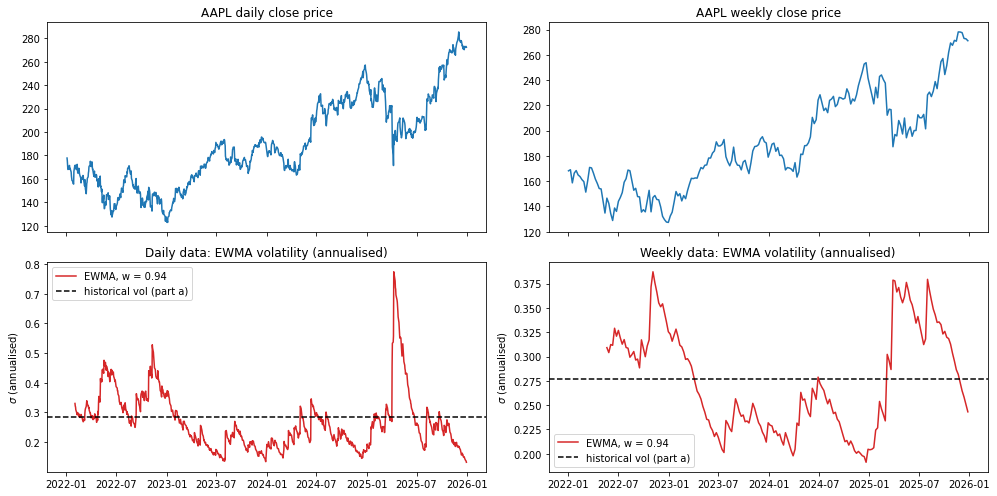
\includegraphics[width=\textwidth]{q4b_ewma.png}
  \caption{Top: AAPL daily (left) and weekly (right) close prices. Bottom: EWMA volatility
  estimates ($w = 0.94$, annualised) and the historical volatility from part~(a).}
  \label{fig:q4b}
\end{figure}

The volatility rises sharply after large price movements and then decays back towards the
historical estimate of part~(a). The most striking example is April 2025, when the daily EWMA
volatility jumps from about 25\% to almost 80\%. The weekly curve is smoother and slower to
react to price spikes: with $w = 0.94$ the effective memory is about $1/(1-w) \approx 17$
observations, i.e.\ about 3.5 weeks for daily data but about 4 months for weekly data. The first
20 observations are only used to compute $\sigma^*$, so each curve starts at the 20th return. The
starting value matters less and less, because its weight shrinks as $w^k$.

\subsection*{(c) Is the asset price model appropriate?}

The model from the lecture (geometric Brownian motion) assumes a \emph{constant} volatility
$\sigma$. Figure~\ref{fig:q4b} clearly contradicts this. The EWMA estimate varies between roughly
13\% and 77\% for daily data and between 19\% and 39\% for weekly data, and it shows volatility
clustering: calm periods (most of 2023--2024) alternate with turbulent periods (2022, April 2025).
The heavy tails in the daily Q-Q plots of Question 1b point in the same direction, since a mixture
of normal distributions with different variances is heavy-tailed. The constant-volatility model is
therefore not fully appropriate for this data, especially at the daily scale and during market
stress. It can still serve as a reasonable first approximation over longer horizons, where the
weekly returns are close to normal and the average volatility is stable (Table~\ref{tab:q4a}).
Models with time-varying volatility (e.g.\ GARCH or stochastic volatility) would describe the data
better.

%======================================================================
\section{Binomial method}
%======================================================================

Parameters: $S_0 = 1.0$, $T = 3.0$, $\mu = r = 0.05$, $\sigma = 0.3$, $E = 1.5$, $M = 12$
($\delta t = 0.25$).

\subsection*{(a) Fixed strike lookback put}

\todo{Not yet in the notebook. Add the solution, code (appendix) and the time-zero price.}

\subsection*{(b) Shout put}

\todo{Not yet in the notebook. Add the solution, code (appendix) and the time-zero price.}

%======================================================================
\appendix
\section{Code}
\label{app:code}
%======================================================================

The code below is the content of \texttt{OVM\_assignment\_1.ipynb}, split per question.
Cells are run in order and share variables.

\subsection{Question 1}

\begin{lstlisting}[caption={Q1a: download and plot the daily close prices.}, label={lst:q1a-price}]
import matplotlib.pyplot as plt
import yfinance as yf

# Download daily prices (end date is exclusive, so we use 1 Sep 2026)
close = yf.Ticker("AAPL").history(start="2025-09-01", end="2026-08-31")["Close"]

plt.figure(figsize=(10, 4))
plt.plot(close)
plt.title("AAPL (*---*) daily close price")
plt.xlabel("Date")
plt.ylabel("Close price (USD)")
plt.tight_layout()
plt.show()
\end{lstlisting}

\begin{lstlisting}[caption={Q1a: daily simple and logarithmic returns.}, label={lst:q1a-returns}]
import numpy as np

# Simple daily return: (P_t - P_{t-1}) / P_{t-1}
daily_return = (close-close.shift(1))/close.shift(1)

# Log daily return: ln(P_t / P_{t-1})
log_return = np.log(close/close.shift(1))

fig, axes = plt.subplots(2, 1, figsize=(10, 6), sharex=True)

axes[0].plot(daily_return)
axes[0].set_title("Daily simple return")
axes[0].set_ylabel("Return")

axes[1].plot(log_return)
axes[1].set_title("Daily logarithmic return")
axes[1].set_xlabel("Date")
axes[1].set_ylabel("Log return")

plt.tight_layout()
plt.show()
\end{lstlisting}

\begin{lstlisting}[caption={Q1b: histogram, sample mean and variance of daily log returns.}, label={lst:q1b-hist}]
log_returns_clean=log_return.dropna()
plt.figure(figsize=(10, 4))
plt.hist(log_returns_clean, bins=50, edgecolor="black")
plt.title("AAPL (*---*) histogram of daily logarithmic returns")
plt.xlabel("Log return")
plt.ylabel("Number of days")
plt.tight_layout()
plt.show()

mean_lr=log_returns_clean.mean()
var_lr=log_returns_clean.var()
sd_lr=np.sqrt(var_lr)

print("Sample mean:", mean_lr)
print("Sample variance:", var_lr)
\end{lstlisting}

\begin{lstlisting}[caption={Q1b: Q-Q plot of daily log returns against $\mathcal N(\hat\mu,\hat\sigma^2)$.}, label={lst:q1b-qq}]
from scipy.stats import norm

# Empirical quantiles (sorted data) vs. normal quantiles at probabilities (k-0.5)/n
sample_q=np.sort(log_returns_clean)
n=len(sample_q)
probabilities=(np.arange(1,n+1)-0.5)/n
theory_q=norm.ppf(probabilities,loc=mean_lr,scale=sd_lr)

plt.figure(figsize=(6, 6))
plt.scatter(theory_q,sample_q,s=10)
plt.plot(theory_q,theory_q,color="red")
plt.title("Q-Q plot: AAPL daily log returns vs N((*$\hat\mu$*), (*$\hat\sigma^2$*))")
plt.xlabel("Theoretical quantiles (normal)")
plt.ylabel("Sample quantiles (log returns)")
plt.tight_layout()
plt.show()
\end{lstlisting}

\begin{lstlisting}[caption={Q1b: daily and weekly log returns 2022--2025, statistics and Q-Q plots.}, label={lst:q1b-weekly}]
close_day = yf.Ticker("AAPL").history(start="2022-01-01", end="2025-12-31")["Close"]
close_week = yf.Ticker("AAPL").history(start="2022-01-01", end="2025-12-31", interval="1wk")["Close"]

day_log_returns=np.log(close_day/close_day.shift(1))
day_log_returns=day_log_returns.dropna()
mean_d=day_log_returns.mean()
var_d=day_log_returns.var()
sd_d=np.sqrt(var_d)

week_log_returns=np.log(close_week/close_week.shift(1))
week_log_returns=week_log_returns.dropna()
mean_w=week_log_returns.mean()
var_w=week_log_returns.var()
sd_w=np.sqrt(var_w)

print("Daily  2022-2025: mean =", mean_d, ", variance =", var_d)
print("Weekly 2022-2025: mean =", mean_w, ", variance =", var_w)

plt.figure(figsize=(10, 4))
plt.hist(week_log_returns, bins=30, edgecolor="black")
plt.title("AAPL - histogram of weekly logarithmic returns (2022-2025)")
plt.xlabel("Log return")
plt.ylabel("Number of weeks")
plt.tight_layout()
plt.show()

# Q-Q plot, daily returns 2022-2025
sample_q=np.sort(day_log_returns)
n=len(sample_q)
probabilities=(np.arange(1,n+1)-0.5)/n
theory_q=norm.ppf(probabilities,loc=mean_d,scale=sd_d)

plt.figure(figsize=(6, 6))
plt.scatter(theory_q,sample_q,s=10)
plt.plot(theory_q,theory_q,color="red")
plt.title("Q-Q plot: AAPL daily log returns vs N((*$\hat\mu$*), (*$\hat\sigma^2$*)) 2022-2025")
plt.xlabel("Theoretical quantiles (normal)")
plt.ylabel("Sample quantiles (log returns)")
plt.tight_layout()
plt.show()

# Q-Q plot, weekly returns 2022-2025
sample_q=np.sort(week_log_returns)
n=len(sample_q)
probabilities=(np.arange(1,n+1)-0.5)/n
theory_q=norm.ppf(probabilities,loc=mean_w,scale=sd_w)

plt.figure(figsize=(6, 6))
plt.scatter(theory_q,sample_q,s=10)
plt.plot(theory_q,theory_q,color="red")
plt.title("Q-Q plot: AAPL weekly log returns vs N((*$\hat\mu$*), (*$\hat\sigma^2$*))")
plt.xlabel("Theoretical quantiles (normal)")
plt.ylabel("Sample quantiles (log returns)")
plt.tight_layout()
plt.show()
\end{lstlisting}

\subsection{Question 2}

\begin{lstlisting}[caption={Q2: basic Monte Carlo estimate of $\mathbb E[1/\sqrt U]$.}, label={lst:q2-basic}]
rng=np.random.default_rng(seed=41)

n=1000

U=rng.uniform(0,1,n)
y=1/np.sqrt(U)

estimate=y.mean()
print("Monte Carlo estimate:", estimate)
print("Absolute error:", abs(estimate - 2))
\end{lstlisting}

\begin{lstlisting}[caption={Q2: estimates and 95\% confidence intervals for $N=10^2,\dots,10^5$.}, label={lst:q2-ci}]
# One MC estimate and its 95% confidence interval for each sample size
Ns=[10**2,10**3,10**4,10**5]
estimates=[]
half_widths=[]

for n in Ns:
    y=1/np.sqrt(rng.uniform(0,1,n))
    est=y.mean()
    se=y.std(ddof=1)/np.sqrt(n)
    estimates.append(est)
    half_widths.append(1.96*se)
    print(f"N={n:>6}: estimate={est:.4f}, 95% CI=[{est-1.96*se:.4f}, {est+1.96*se:.4f}]")

plt.figure(figsize=(8, 4))
plt.errorbar(Ns,estimates,yerr=half_widths,fmt="o",capsize=5,label="MC estimate with 95% CI")
plt.axhline(2,color="red",linestyle="--",label="exact value = 2")
plt.xscale("log")
plt.title("MC estimates of $E[1/\sqrt{U}]$ with 95% confidence intervals")
plt.xlabel("Number of samples N")
plt.ylabel("Estimate")
plt.legend()
plt.tight_layout()
plt.show()
\end{lstlisting}

\begin{lstlisting}[caption={Q2: $M=1000$ repetitions per $N$, error distribution, CI coverage and convergence plot.}, label={lst:q2-repeat}]
# Repeat the MC experiment M times for each N to study the distribution of the error
M=1000
errors={}
coverage={}

for n in Ns:
    err=np.empty(M)
    inside=0
    for m in range(M):
        y=1/np.sqrt(rng.uniform(0,1,n))
        est=y.mean()
        se=y.std(ddof=1)/np.sqrt(n)
        err[m]=est-2
        inside+=abs(est-2)<=1.96*se
    errors[n]=err
    coverage[n]=inside/M
    print(f"N={n:>6}: mean |error|={np.abs(err).mean():.5f}, CI coverage={coverage[n]:.3f}")

mean_abs_err=[np.abs(errors[n]).mean() for n in Ns]

plt.figure(figsize=(8, 4))
plt.loglog(Ns,mean_abs_err,"o-",label="mean |error| (MC)")
plt.loglog(Ns,mean_abs_err[0]*np.sqrt(Ns[0])/np.sqrt(Ns),"--",color="red",label="reference slope $N^{-1/2}$")
plt.title("Speed of convergence of the MC estimator")
plt.xlabel("Number of samples N")
plt.ylabel("Mean absolute error")
plt.legend()
plt.tight_layout()
plt.show()
\end{lstlisting}

\begin{lstlisting}[caption={Q2: histograms with fitted normal density and Q-Q plots of the errors.}, label={lst:q2-normality}]
# Histogram of errors with fitted normal density (top) and Q-Q plot vs fitted normal (bottom)
fig, axes = plt.subplots(2, 4, figsize=(16, 7))

for j, n in enumerate(Ns):
    err=errors[n]
    mu=err.mean()
    sd=err.std(ddof=1)

    x=np.linspace(err.min(),err.max(),400)
    axes[0, j].hist(err,bins=50,density=True,edgecolor="black")
    axes[0, j].plot(x,norm.pdf(x,loc=mu,scale=sd),color="red")
    axes[0, j].set_title(f"Errors, N = {n}")
    axes[0, j].set_xlabel("Error")

    sample_q=np.sort(err)
    probabilities=(np.arange(1,M+1)-0.5)/M
    theory_q=norm.ppf(probabilities,loc=mu,scale=sd)
    axes[1, j].scatter(theory_q,sample_q,s=8)
    axes[1, j].plot(theory_q,theory_q,color="red")
    axes[1, j].set_title(f"Q-Q plot, N = {n}")
    axes[1, j].set_xlabel("Theoretical quantiles (normal)")
    axes[1, j].set_ylabel("Sample quantiles (errors)")

plt.tight_layout()
plt.show()
\end{lstlisting}

\subsection{Question 3}

\begin{lstlisting}[caption={Q3a: one path of the discrete price model, $L=5$.}, label={lst:q3a-path}]
np.random.seed(41)

S0, sigma, mu, T = 170, 0.344, 0.1, 1

L=5
dt=T/L

S=[S0]

# S(t_{i+1}) = S(t_i) * (1 + mu*dt + sigma*sqrt(dt)*Z)
for i in range(L):
    z=np.random.randn()
    S_next=S[-1]*(1+mu*dt+sigma*np.sqrt(dt)*z)
    S.append(S_next)

t=np.arange(L+1)*dt
plt.plot(t, S, marker='o')
plt.xlabel('t'); plt.ylabel('S(t)')
plt.title('One simulated price path, L = 5')
plt.show()
\end{lstlisting}

\begin{lstlisting}[caption={Q3a: $M=5000$ simulations of $S_T$ and histogram for $L=5$.}, label={lst:q3a-hist}]
# Simulate M paths at once (vectorised over paths) and return S_T
def simulate_ST(L,M=5000):
    dt=T/L
    S=np.full(M,S0,dtype=float)
    for i in range(L):
        z=np.random.randn(M)
        S=S*(1+mu*dt+sigma*np.sqrt(dt)*z)
    return S

ST=simulate_ST(5)
plt.hist(ST, bins=50, density=True)
plt.xlabel('S_T'); plt.title('Histogram of S_T, L = 5')
plt.show()
\end{lstlisting}

\begin{lstlisting}[caption={Q3a: empirical CDFs of $S_T$ for $L=5,\dots,100$ vs.\ the theoretical log-normal CDF.}, label={lst:q3a-ecdf}]
plt.figure(figsize=(18, 6))

np.random.seed(41)

LS=[5,10,20,50,100]

for L in LS:
    ST=np.sort(simulate_ST(L))
    edcf=np.arange(1,len(ST)+1)/len(ST)
    plt.step(ST,edcf,where='post',label=f'L={L}')

# Theoretical CDF: ln(S_T/S0) ~ N((mu - sigma^2/2) T, sigma^2 T)
x=np.linspace(50,450,500)
F=norm.cdf((np.log(x/S0)-(mu-0.5*sigma**2)*T)/(sigma*np.sqrt(T)))
plt.plot(x, F, 'k--', linewidth=2, label='Theoretical')
plt.xlabel('S_T'); plt.ylabel('F(x)')
plt.title('Empirical CDFs of S_T vs theoretical CDF')
plt.legend(); plt.show()
\end{lstlisting}

\begin{lstlisting}[caption={Q3b: standard MC vs.\ antithetic variables for $\mathbb E[S_T]$.}, label={lst:q3b}]
S0, sigma, mu, T = 170, 0.344, 0.1, 1
exact=S0*np.exp(mu*T)
rng=np.random.default_rng(seed=41)

ms=[10**2,10**3,10**4,10**5]

# Exact solution of the continuous-time model for given Z
def ST_exact(z):
    return S0*np.exp((mu-0.5*sigma**2)*T+sigma*np.sqrt(T)*z)

print(f"E[S_T]={exact:.4f}")

for m in ms:
    # standard MC with m samples
    z=rng.standard_normal(m)
    y=ST_exact(z)
    est=y.mean()
    hw=1.96*y.std(ddof=1)/np.sqrt(m)

    # antithetic: m/2 pairs (Z, -Z), i.e. the same number m of evaluations
    z2=z[:m//2]
    y2=0.5*(ST_exact(z2)+ST_exact(-z2))
    est2=y2.mean()
    hw2=1.96*y2.std(ddof=1)/np.sqrt(m//2)

    print(f"M={m:>6}: MC = {est:.3f}, CI=[{est-hw:.3f}, {est+hw:.3f}] | "
          f"AMC = {est2:.3f}, CI=[{est2-hw2:.3f}, {est2+hw2:.3f}] | "
          f"I_M/I_AM = {hw/hw2:.3f}")
\end{lstlisting}

\subsection{Question 4}

\begin{lstlisting}[caption={Q4a: historical volatility from daily and weekly data.}, label={lst:q4a}]
sigma_d=day_log_returns.std()
sigma_w=week_log_returns.std()

# Annualise: sigma = s / sqrt(dt), dt = 1/252 (daily) or 1/52 (weekly)
sigma_d_anum=sigma_d*np.sqrt(252)
sigma_w_anum=sigma_w*np.sqrt(52)

print(f"Daily:  sigma per day  = {sigma_d:.5f}, annualised = {sigma_d_anum:.4f}")
print(f"Weekly: sigma per week = {sigma_w:.5f}, annualised = {sigma_w_anum:.4f}")
\end{lstlisting}

\begin{lstlisting}[caption={Q4b: EWMA volatility estimates ($w=0.94$, first 20 observations for $\sigma^*$).}, label={lst:q4b}]
import pandas as pd

# sigma_n^2 = w * sigma_{n-1}^2 + (1-w) * u_n^2, started from the sample variance of the first n_init returns
def ewma(returns, w=0.94, n_init=20):
    u=returns.values
    var=np.full(len(u),np.nan)
    var[n_init-1]=np.var(u[:n_init],ddof=1)
    for i in range(n_init,len(u)):
        var[i]=w*var[i-1]+(1-w)*u[i]**2
    return pd.Series(np.sqrt(var),index=returns.index)

vol_d = ewma(day_log_returns)  * np.sqrt(252)   # annualised daily-data estimate
vol_w = ewma(week_log_returns) * np.sqrt(52)    # annualised weekly-data estimate
fig, axes = plt.subplots(2, 2, figsize=(14, 7), sharex="col")

axes[0, 0].plot(close_day)
axes[0, 0].set_title("AAPL daily close price")
axes[1, 0].plot(vol_d, color="tab:red", label="EWMA, w = 0.94")
axes[1, 0].axhline(day_log_returns.std() * np.sqrt(252), color="k", ls="--",
                   label="historical vol (part a)")
axes[1, 0].set_title("Daily data: EWMA volatility (annualised)")
axes[1, 0].legend()
axes[0, 1].plot(close_week)
axes[0, 1].set_title("AAPL weekly close price")
axes[1, 1].plot(vol_w, color="tab:red", label="EWMA, w = 0.94")
axes[1, 1].axhline(week_log_returns.std() * np.sqrt(52), color="k", ls="--",
                   label="historical vol (part a)")
axes[1, 1].set_title("Weekly data: EWMA volatility (annualised)")
axes[1, 1].legend()
for ax in axes[1]:
    ax.set_ylabel(r"$\sigma$ (annualised)")
plt.tight_layout()
plt.show()
\end{lstlisting}

\subsection{Question 5}

\todo{Add the binomial-method code for the lookback put and the shout put.}

\end{document}
